\documentclass[conference]{IEEEtran}
\IEEEoverridecommandlockouts

\usepackage{cite}
\usepackage{amsmath,amssymb,amsfonts}
\usepackage{graphicx}
\usepackage{textcomp}
\usepackage{xcolor}
\usepackage{booktabs}
\usepackage{algorithm}
\usepackage{algpseudocode}
\usepackage{tikz}
\usetikzlibrary{arrows.meta,positioning,shapes.geometric}
\usepackage{listings}
\usepackage{caption}
\usepackage{subcaption}

\graphicspath{{figures/}}

\lstdefinelanguage{json}{
    basicstyle=\ttfamily\scriptsize,
    showstringspaces=false,
    breaklines=true,
    frame=single,
    literate=
     *{0}{{{\color{blue}0}}}{1}
      {1}{{{\color{blue}1}}}{1}
      {2}{{{\color{blue}2}}}{1}
      {3}{{{\color{blue}3}}}{1}
      {4}{{{\color{blue}4}}}{1}
      {5}{{{\color{blue}5}}}{1}
      {6}{{{\color{blue}6}}}{1}
      {7}{{{\color{blue}7}}}{1}
      {8}{{{\color{blue}8}}}{1}
      {9}{{{\color{blue}9}}}{1}
}

\begin{document}

\title{Zero-Touch Federated Learning Attacks: An LLM-Directed Reinforcement-Learning\\ Attacker Benchmarked Against FLTrust and Byzantine-Robust Defenses}

\author{
\IEEEauthorblockN{Author 1 Name}
\IEEEauthorblockA{\textit{Department or Affiliation} \\
\textit{Institution Name}\\
City, Country \\
Email Address}
\and
\IEEEauthorblockN{Author 2 Name}
\IEEEauthorblockA{\textit{Department or Affiliation} \\
\textit{Institution Name}\\
City, Country \\
Email Address}
}

\maketitle

\begin{abstract}
Federated learning (FL) aggregates client model updates into a shared global model without inspecting raw client data, so the server cannot verify that a submitted update reflects honest training. Byzantine-robust defenses such as FLTrust, Multi-Krum, and DnC guard against this with a fixed, hand-designed notion of what a poisoned update looks like, while a real attacker can keep adapting. We present a zero-touch attacker for FL: an LLM policy, trained with reinforcement learning rather than a hand-authored attack script, that decides each round which of its controllable clients to poison and how to compose a small set of primitive weight operators into a poisoned update. The policy is trained online with Group-Relative Policy Optimization (GRPO) against a verifiable reward that credits accuracy degradation and evasion while discouraging wasteful or easily-detected (Sybil-like) client use, using a freeze-and-alternate schedule against a co-trained defender LLM. We evaluate the trained attacker in a benchmark that replays its committed actions, unchanged, against a panel of independent defenses -- undefended FedAvg, FLTrust, Multi-Krum, DnC, DeFL, and the co-trained LLM defender -- so that the defense, not the attack, is the only thing that varies. In a preliminary 50-round run, the attack collapses undefended FedAvg and the co-trained LLM defender to near-random accuracy, is fully neutralized by Multi-Krum and FLTrust, and causes substantial damage against DeFL despite DeFL's comparatively strong detection rate. We report this as a preliminary, single-run result alongside the full system design, pending broader replication.
\end{abstract}

\begin{IEEEkeywords}
federated learning, model poisoning, large language models, reinforcement learning, Group-Relative Policy Optimization, Byzantine-robust aggregation, FLTrust, adversarial machine learning
\end{IEEEkeywords}

\section{Introduction}

Federated learning (FL) lets edge devices collaboratively train a shared model without exposing local data \cite{fedavg}. Each round, a central server broadcasts the global model, every client trains locally, and the server aggregates the returned updates -- typically by Federated Averaging (FedAvg) -- into a new global model. Because the server sees only model updates, it has no independent way to check that a given update reflects honest training, and a subset of compromised clients can submit manipulated updates that degrade the global model's accuracy \cite{bagdasaryan2020,bhagoji2019}.

The dominant defense strategy treats an update as a point in a high-dimensional vector space and looks for statistical outliers: coordinate-wise median and trimmed mean bound the influence of any single coordinate \cite{byzantine}; Multi-Krum keeps the updates closest to their neighbors under an $\ell_2$ distance \cite{krum}; DnC projects updates onto their top spectral direction and drops the ones that stick out furthest along it \cite{dnc}; FLTrust bootstraps a trusted reference update from a small clean root set held by the server and rescales client updates toward it by cosine trust \cite{fltrust}; FoolsGold penalizes clients whose updates look like each other's clones \cite{foolsgold}; and DeFL tracks how a model's per-layer gradient-norm profile evolves across rounds, flagging clients whose layer-wise contribution deviates from the group during a critical learning period \cite{defl}. Each of these encodes a fixed assumption about attacker behavior -- outlier norm, distance from the bulk, a dominant spectral signature, or a divergent per-layer profile -- baked in once at design time. An attacker aware of the deployed rule can construct an update that satisfies its assumption while still corrupting the aggregate \cite{fang2020}, but doing so by hand requires a human to re-derive an evasion strategy every time the defense changes -- an arms race that, historically, has been fought on the timescale of publications rather than training rounds.

This paper asks whether that process can instead be automated: can an attacker \emph{learn}, through interaction and a verifiable reward alone, which of its controllable clients to poison and how to compose primitive weight edits into an update that both damages the global model and evades detection -- with no attack template, target heuristic, or hand-derived evasion rule supplied in advance? We build this attacker inside \emph{Zero-Touch Federated Learning}, a testbed in which the attack is generated directly by an LLM policy trained with reinforcement learning. The attacker is a \emph{partial insider}: it controls a fixed minority pool of clients and, each round, is given dimensionless statistics of its own controllable clients' honest updates -- never a cross-client reference, another client's update, or any defense's internal state -- and must decide which, and how many, of its clients to recruit and an ordered plan of primitive operators to apply to each. A deterministic interpreter applies the plan; the attacker never touches raw weights directly. The policy is trained online with GRPO \cite{grpo} against an exactly verifiable, continuous reward computed from ground truth available only at training time: the accuracy drop the committed action caused, how confidently a defender judged the poisoned clients malicious, whether the plan parsed, how many clients were used, and -- when more than one client is used -- how distinct their individual contributions are from one another.

Because the attacker never observes any defense's internal features, thresholds, or verdicts beyond the aggregate accuracy signal it trains against, we can ask a transfer question that a co-adapted attacker/defender pair alone cannot answer: does a policy trained only against a co-evolving LLM defender's accuracy and confidence signal produce an attack that \emph{also} degrades accuracy under classical, non-learned robust aggregators it never saw during training? We answer this with a fixed-attack, varied-defense benchmark harness that replays one committed attack plan per round against FedAvg, an Oracle upper bound, FLTrust, Multi-Krum, DnC, DeFL, and the co-trained LLM defender, each maintaining its own independent global model, so that the defense is the only variable across the comparison.

\textbf{Contributions.} This paper makes the following contributions:
\begin{itemize}
    \item A zero-touch FL attacker in which client selection and weight-operator composition are generated directly by an LLM policy, using a general-purpose primitive-operator DSL, without prescribing any attack strategy in advance.
    \item A verifiable, continuous reward that jointly credits accuracy degradation and evasion (stealth) while penalizing malformed output, the use of more controllable clients than necessary, and non-diverse (Sybil-like) multi-client collusion -- derived directly from ground-truth knowledge of the poisoned set available only during training.
    \item A GRPO training protocol -- freeze-and-alternate scheduling, stochastic opponent scoring, and an opponent league -- that keeps the attacker's learning signal alive against a co-evolving LLM defender and formalizes the interaction as a Stackelberg game.
    \item A \emph{fixed-attack, varied-defense benchmark harness} that replays one committed attack plan per round against a panel of independently evolving defenses (FedAvg, Oracle, FLTrust, Multi-Krum, DnC, DeFL, and the co-trained LLM defender), isolating the defense as the only variable and testing whether the learned evasion strategy transfers to defenses the attacker never trained against.
    \item A complete open system design covering the attacker contract, reward, training schedule, defense panel, and benchmark protocol -- a reusable testbed for studying autonomous, LLM-directed FL attacks against both learned and classical Byzantine-robust defenses.
\end{itemize}

The remainder of this paper is organized as follows. Section~\ref{sec:related} surveys robust FL aggregation, adaptive poisoning attacks, and LLM RL fine-tuning methods. Section~\ref{sec:threat} defines the threat model, including the black-box relationship between the attacker and the benchmarked defenses. Section~\ref{sec:attack} details the attack mechanism: the two-phase protocol, the attacker's client-selection and DSL contract, and the defender it co-trains against. Section~\ref{sec:rl} describes the GRPO training methodology and the verifiable reward. Section~\ref{sec:setup} describes the experimental setup, including the defense panel and the benchmark protocol. Section~\ref{sec:results} reports a preliminary benchmark run of the trained attacker against the full defense panel and discusses what it does and does not reveal about detection quality versus realized protection. Section~\ref{sec:conclusion} concludes and outlines future work.

\begin{figure*}[t]
\centering
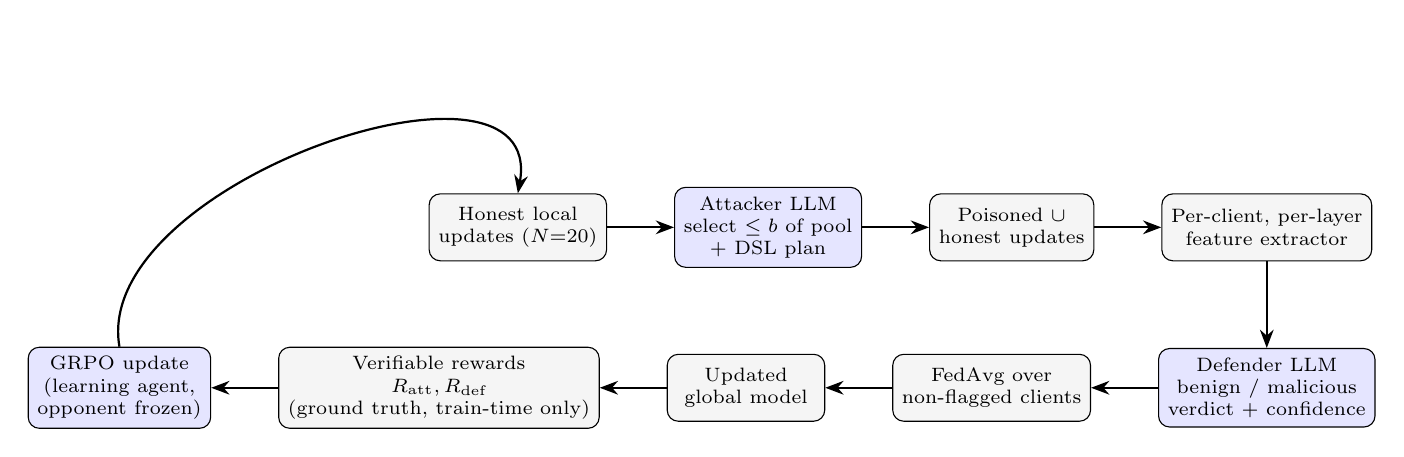
\begin{tikzpicture}[
    node distance=0.55cm and 0.85cm,
    every node/.style={font=\scriptsize},
    box/.style={draw, rounded corners, align=center, minimum height=0.85cm, minimum width=2.0cm, fill=gray!8},
    llmbox/.style={box, fill=blue!10},
    arr/.style={-Stealth, thick}
]
\node[box] (clients) {Honest local\\updates ($N{=}20$)};
\node[llmbox, right=of clients] (att) {Attacker LLM\\select $\le b$ of pool\\ + DSL plan};
\node[box, right=of att] (combine) {Poisoned $\cup$\\honest updates};
\node[box, right=of combine] (feat) {Per-client, per-layer\\feature extractor};

\node[llmbox, below=1.1cm of feat] (def) {Defender LLM\\benign / malicious\\verdict + confidence};
\node[box, left=of def] (agg) {FedAvg over\\non-flagged clients};
\node[box, left=of agg] (global) {Updated\\global model};
\node[box, left=of global] (reward) {Verifiable rewards\\$R_{\text{att}},R_{\text{def}}$\\(ground truth, train-time only)};
\node[llmbox, left=of reward] (grpo) {GRPO update\\(learning agent,\\opponent frozen)};

\draw[arr] (clients) -- (att);
\draw[arr] (att) -- (combine);
\draw[arr] (combine) -- (feat);
\draw[arr] (feat) -- (def);
\draw[arr] (def) -- (agg);
\draw[arr] (agg) -- (global);
\draw[arr] (global) -- (reward);
\draw[arr] (reward) -- (grpo);
\draw[arr] (grpo.north) to[out=100,in=80] (clients.north);
\end{tikzpicture}
\caption{One Phase-2 training round. The attacker LLM selects which controllable clients to poison and composes a per-client DSL plan; the defender best-responds from statistical features alone; FedAvg aggregates the non-flagged clients; and ground-truth-derived rewards drive a GRPO update for whichever agent is currently learning while the other remains frozen. At benchmark time (Section~\ref{sec:setup}) the same committed attacker action is instead replayed, unmodified, against a panel of classical defenses in place of the co-trained defender.}
\label{fig:architecture}
\end{figure*}

\section{Related Work}
\label{sec:related}

\subsection{Federated Learning and the Poisoning Attack Surface}
In a standard FL round, a central server distributes the global model to $N$ clients, each performs local training, and the server aggregates the returned updates through FedAvg \cite{fedavg}. Model poisoning occurs when compromised clients submit manipulated updates. Untargeted attacks degrade overall accuracy, whereas targeted (backdoor) attacks introduce a narrower vulnerability while leaving overall accuracy largely intact \cite{bagdasaryan2020}; this paper focuses on the untargeted case -- driving down the global model's overall test accuracy while evading detection. Non-IID data partitioning, common in real deployments, makes detection harder in either case, because an honest client's update can legitimately look like a statistical outlier when its local data distribution differs from the majority.

\subsection{Byzantine-Robust and Statistical Defenses}
Coordinate-wise median and trimmed-mean aggregation give provable robustness under a bounded number of Byzantine clients by bounding the influence of any one coordinate \cite{byzantine}. Krum and Multi-Krum score each client by its summed squared distance to its closest neighbors under a Euclidean-distance criterion and keep only the most central updates \cite{krum}. DnC instead treats poisoning as a spectral outlier problem: it centers the client updates, projects them onto the top right singular vector of the centered matrix, and removes the clients whose projection along it is largest \cite{dnc}. FLTrust bootstraps a trusted direction from a small clean root dataset held by the server, scores each client by the ReLU of its cosine similarity to that direction, rescales surviving updates to the trusted update's magnitude, and combines them in a trust-weighted average \cite{fltrust}. FoolsGold instead exploits update \emph{similarity across clients}, down-weighting clients whose contribution histories are pairwise similar -- the Sybil/collusion signature \cite{foolsgold}. DeFL departs from these per-round, whole-update statistics: it tracks a Federated Gradient Norm Vector per layer across rounds, detects a Critical Learning Period from a jump in the aggregate per-layer gradient norm, and votes a client malicious via an adaptive per-layer outlier threshold \cite{defl}. Every method in this family encodes, once, a fixed geometric or statistical prior about what a poisoned update looks like.

\subsection{Adaptive and Learning-Based Attacks}
A growing body of work shows that an attacker aware of the deployed defense can construct updates that satisfy its assumptions while still corrupting the aggregate. Fang~et~al.\ formulate local model poisoning as an optimization problem that directly targets a known Byzantine-robust aggregation rule \cite{fang2020}. Bhagoji~et~al.\ show that a single persistent attacker using boosted updates can substantially bias the global model even under conventional defenses \cite{bhagoji2019}. These findings motivate an attacker that learns an evasion strategy against the defense it currently faces instead of relying on a hand-derived attack tuned to one fixed aggregation rule; unlike these prior adaptive attacks, the attacker studied here has no white-box access to any defense's parameters, thresholds, or intermediate scores -- it observes interaction outcomes only through the RL reward signal computed from the resulting global-model accuracy and, when co-training against the LLM defender, its confidence.

\subsection{Fine-Tuning and Alignment of Large Language Models}
LLMs are commonly aligned or specialized with reinforcement learning from a scalar or preference signal. Proximal Policy Optimization (PPO) trains a policy with a learned value/critic network for per-token credit assignment and has been widely used for instruction-following alignment \cite{ppo,ouyang2022}. Direct Preference Optimization (DPO) learns from pairwise preference data without an explicit reward model or online rollout \cite{dpo}, but it operates offline and does not use the magnitude of an exactly computable reward. Group-Relative Policy Optimization (GRPO) samples $G$ completions per state, assigns each an exactly verifiable scalar reward, and uses the normalized reward within the group as the advantage for a policy-gradient update \cite{grpo}. This critic-free formulation suits our setting because each round yields one terminal reward based on the ground-truth poisoned set, the resulting accuracy, and the defender's confidence. Parameter-efficient fine-tuning through Low-Rank Adaptation (LoRA) \cite{lora2022} and its 4-bit quantized form, QLoRA \cite{qlora2023}, allows the attacker and defender to use small adapters over one shared frozen base model (Section~\ref{sec:setup}).

\section{Threat Model}
\label{sec:threat}

We adopt a \emph{partial-insider} threat model for the attacker.

\textbf{Attacker capabilities.} The attacker controls a fixed, strict-minority pool of $n_{\mathrm{compromisable}}$ clients (default 5 of $N=20$) across the entire run. In any given round it may poison at most $b=\min(\text{budget}, n_{\mathrm{compromisable}})$ of that pool, where the budget is drawn stochastically during training and fixed at evaluation time. For each pool client, the attacker observes per-layer statistics of that client's \emph{own honest update} relative to the current global model (Section~\ref{sec:attacker-contract}). It does not receive a robust reference such as the coordinate-wise median, another client's update, or a statistic computed over the pool. The attacker cannot see any defense's internal state (features, thresholds, trust scores, or verdicts), alter the server's aggregation code, or inject clients outside its fixed pool.

\textbf{Defense visibility.} During training, the attacker is optimized only against the resulting global-model accuracy and, when co-training against the frozen LLM defender, the defender's confidence on the poisoned clients (Section~\ref{sec:rewards}) -- it never sees the defender's per-client features or verdicts in its own prompt. At evaluation time, the trained (frozen) attacker's committed action is replayed unmodified against every defense in the benchmark panel (Section~\ref{sec:defense-panel}); the attacker never trains against, and has no visibility into, the classical defenses (FLTrust, Multi-Krum, DnC, DeFL). Any resulting damage those defenses fail to fully mitigate is therefore a transfer property of the learned strategy, not a result of the attacker adapting to them directly.

\textbf{Out of scope.} We do not model network-level attacks, Sybil attacks that fabricate new client identities, data-poisoning attacks mounted at a client's local training data, targeted/backdoor objectives, or collusion between the attacker and a compromised aggregation server. These are natural extensions of the testbed (Section~\ref{sec:conclusion}) but are not evaluated here.

\section{Attack Mechanism}
\label{sec:attack}

\subsection{Model and Data Environment}
The environment simulates FL on MNIST with $N=20$ clients under a non-IID partition using the FLTrust-style bias-$q$ scheme, in which each client's local data is skewed toward a subset of classes with bias strength $q$ \cite{fltrust}. The global model is a lightweight multilayer perceptron (MLP) with 970 parameters (\texttt{AvgPool2d(4)} $\to$ \texttt{Linear(49,16)} $\to$ \texttt{ReLU} $\to$ \texttt{Linear(16,10)}). At this scale, per-layer statistics provide a compact observation an LLM can process as structured JSON rather than raw tensors, while the model still contains distinct weight and bias tensors the attacker can target selectively.

\subsection{Two-Phase Protocol}
\textbf{Phase 1 (honest training).} All $N$ clients train honestly via FedAvg for a configured number of rounds. The resulting global model, each client's locally trained weights, and the baseline test accuracy are checkpointed and form the starting state for Phase 2.

\textbf{Phase 2 (adversarial arms race).} A Stackelberg game begins. The attacker moves first each round, and the defender best-responds to the resulting mixture of poisoned and honest updates. Figure~\ref{fig:architecture} illustrates one round, and Algorithm~\ref{alg:round} gives the corresponding pseudocode.

\begin{algorithm}[t]
\caption{Phase-2 Stackelberg Round}
\label{alg:round}
\begin{algorithmic}[1]
\Require global model $G_{t}$, benign client references, controllable pool $P$, budget range
\State $b \sim \mathrm{budget\ distribution}$ (fixed at eval time)
\ForAll{clients $i = 1 \dots N$}
    \State compute honest update $\Delta_i = \mathrm{LocalTrain}(G_t) - G_t$
\EndFor
\State $S_{\text{att}} \gets$ Attacker LLM$(t, P, b, \{\mathrm{stats}(\Delta_i)\}_{i\in P}, \mathrm{acc}_{t-1}, \mathrm{goal})$
\Comment{$S_{\text{att}}$: chosen ids $\subseteq P$, $|S_{\text{att}}|\le b$, + per-client DSL plan}
\ForAll{$i \in S_{\text{att}}$}
    \State $w_i^{\text{poison}} \gets \mathrm{ApplyPlan}(w_i^{\text{benign}}, \mathrm{plan}_i)$
\EndFor
\State $U \gets \{w_i^{\text{poison}} : i \in S_{\text{att}}\} \cup \{w_i^{\text{benign}} : i \notin S_{\text{att}}\}$
\State $F \gets \mathrm{FeatureExtractor}(U, G_t)$
\Comment{features only, no ground truth}
\State $V \gets$ Defender LLM$(F)$
\Comment{$V_i \in \{\mathrm{benign}, \mathrm{malicious}\}$, confidence $c_i$}
\State $G_{t+1} \gets \mathrm{FedAvg}(\{w_i \in U : V_i = \mathrm{benign}\})$
\Comment{keep $G_t$ if all flagged}
\State $\mathrm{acc}_t \gets \mathrm{Evaluate}(G_{t+1})$
\State $R_{\text{att}} \gets \mathrm{AttackerReward}(\mathrm{acc}_{t-1}, \mathrm{acc}_t, S_{\text{att}}, V)$
\State $R_{\text{def}} \gets \mathrm{DefenderReward}(V, S_{\text{att}})$
\Comment{ground truth $=S_{\text{att}}$}
\State GRPO-update the currently learning agent using $R_{\text{att}}$ or $R_{\text{def}}$; opponent frozen
\end{algorithmic}
\end{algorithm}

\subsection{Attacker Contract}
\label{sec:attacker-contract}
\textbf{Input.} The attacker observes the round number, current global accuracy, an attack goal (\texttt{untargeted\_degrade}, evaluated in this paper -- lower global test accuracy by a target amount -- or \texttt{slow\_degrade}, a lower-magnitude per-round variant), the controllable client pool $P$, and round budget $b$. For each pool client's honest update $\Delta = \mathrm{local} - \mathrm{global}$, the observation includes relative update norm $\|\Delta\|/\|G\|$, RMS delta, energy fraction, sign-flip fraction, standard-deviation ratio, absolute-mean ratio, and whole-model cosine similarity to the global model. These are normalized only against the global model; median, mean, and cross-client references remain unavailable to the partial insider. This representation is dimensionless, architecture independent, and unaffected by the round budget.

\textbf{Output.} A single JSON object selecting at most $b$ pool clients and assigning each an ordered attack plan. Table~\ref{tab:ops} lists the ten primitive operators available in the DSL; a deterministic interpreter (not the LLM) applies each plan in order to that client's benign weights, clamps the result to $\pm w_{\max}$, and scrubs any NaN/Inf values. Each operator applies to \texttt{"all"}, a named layer group (e.g.\ \texttt{"net.2"}), or a full parameter key (e.g.\ \texttt{"net.4.weight"}). Listing~\ref{lst:attacker} shows the output schema.

\begin{table}[t]
\caption{Attack operator DSL with 10 primitives. Each operator applies to \texttt{"all"}, a layer group, or a full parameter key.}
\label{tab:ops}
\centering
\small
\begin{tabular}{@{}ll@{}}
\toprule
\textbf{Operator} & \textbf{Effect} \\
\midrule
\texttt{scale} & multiply targeted weights by a factor \\
\texttt{sign\_flip} & negate the top fraction (by magnitude) \\
\texttt{add\_gaussian\_noise} & add $\mathcal{N}(0,\sigma^2)$ per coordinate \\
\texttt{mask} & zero a fraction (largest / smallest / random) \\
\texttt{clip} & clamp values to $\pm v$ \\
\texttt{add\_constant} & additive shift \\
\texttt{permute} & randomly shuffle coordinates \\
\texttt{scale\_neurons} & scale a fraction of highest-norm output rows \\
\texttt{blend\_random} & convex-blend with scaled random noise, $\alpha$ \\
\texttt{quantize} & round to a fixed step size \\
\bottomrule
\end{tabular}
\end{table}

\begin{lstlisting}[language=json, caption={Illustrative attacker output schema (values are illustrative, not measured).}, label={lst:attacker}]
{
  "clients": [
    {
      "id": 3,
      "operations": [
        {"op": "sign_flip", "target": "net.4.weight",
         "fraction": 0.6},
        {"op": "scale", "target": "all", "factor": 1.4}
      ]
    }
  ]
}
\end{lstlisting}

\subsection{The Co-Trained Defender}
\label{sec:defender-contract}
During training, the attacker's opponent is a defender LLM that observes per-client, per-layer statistical features -- $\ell_2$ norm, relative norm vs.\ the coordinate-wise median, cosine similarity to the median, sign agreement with the median, and whole-model features including cosine to the mean (FLTrust-style), max pairwise cosine (FoolsGold-style), and a spectral outlier score (DnC-style) -- and returns a per-client \texttt{is\_suspicious} verdict with a confidence in $[0,1]$. The server FedAvg-aggregates only the clients not flagged as suspicious; if every client is flagged, the previous global model is retained. This gives the attacker a moving, co-adapting opponent to train against (Section~\ref{sec:rl}); Section~\ref{sec:defense-panel} additionally uses the trained defender adapter, frozen, as one entry in the benchmark panel the attacker is evaluated against alongside the classical defenses.

\section{Reinforcement Learning Methodology}
\label{sec:rl}

\subsection{Why GRPO}
The reward available at the end of each Phase-2 round is an exactly computable scalar for both agents (Section~\ref{sec:rewards}), placing the task in the reinforcement learning with verifiable rewards (RLVR) regime. DPO discards reward magnitude and requires an offline preference dataset, neither of which fits an online interaction with a continuously evolving opponent. PPO uses a learned critic for per-token credit assignment along a trajectory. In this setting, however, each agent emits one terminal structured output per round, so a per-token value function offers limited benefit. GRPO samples $G$ completions per environment state, scores them with the verifiable reward, and normalizes the scores within the group to obtain the advantage without a critic network.

\subsection{GRPO Update}
For a group of $G$ sampled completions $\{o_1,\dots,o_G\}$ with rewards $\{r_1,\dots,r_G\}$, the group-normalized advantage is
\begin{equation}
A_i = \frac{r_i - \mathrm{mean}(r)}{\mathrm{std}(r) + \epsilon}.
\label{eq:advantage}
\end{equation}
When $\mathrm{std}(r) < \epsilon$, the group is treated as having zero advantage. Every $A_i$ is set to 0, and the fraction of such groups is logged as a stalled-gradient signal (Section~\ref{sec:opponent-scoring}). The policy is updated by
\begin{equation}
\mathcal{L} = \frac{1}{G}\sum_{i=1}^{G}\Big[-A_i \cdot \overline{\log \pi_\theta(o_i)} + \beta \cdot \overline{\mathrm{KL}}(\pi_\theta \,\|\, \pi_{\mathrm{ref}})_i\Big],
\label{eq:grpo-loss}
\end{equation}
where the bar denotes the mean over generated tokens, $\pi_{\mathrm{ref}}$ is the frozen base model (LoRA adapters disabled) evaluated with the k3 KL estimator, and $\beta$ controls the strength of the KL penalty. Because updates are single-iteration, no PPO-style clipping term is required.

\subsection{Verifiable Continuous Rewards}
\label{sec:rewards}
Both rewards are continuous rather than binary because the GRPO advantage in Eq.~\eqref{eq:advantage} becomes zero when every sampled rollout in a group receives the same reward. This failure mode is particularly likely in the small, nearly binary action spaces associated with choosing clients to flag or poison.

\textbf{Attacker reward.}
\begin{equation}
R_{\mathrm{att}} = \alpha \cdot \mathrm{clip}\!\left(\frac{\Delta A}{\tau_a}, -0.5, 1.5\right) + \beta S - \gamma M - \delta C + \zeta D,
\label{eq:attacker_reward}
\end{equation}
where $\Delta A = \mathrm{acc}_{t-1} - \mathrm{acc}_t$ is the induced accuracy drop and $\tau_a$ (\texttt{target\_accuracy\_drop}, default 0.20) is the target drop for the \texttt{untargeted\_degrade} goal; $S \in [0,1]$ is a continuous stealth term, the mean over the chosen clients of $1-\hat p(\mathrm{malicious})$, where $\hat p$ maps a defender verdict to a soft probability via $\hat p = 0.5 \pm 0.5\cdot\mathrm{confidence}$ (sign depending on the flag); $M$ is the fraction of chosen clients whose plan was malformed or unparseable; $C=(n_{\mathrm{used}}-1)/(|P|-1)$ is a use-fewer-clients penalty, zero for a single-client attack; and $D\in[0,1]$ is a collaboration/diversity bonus, $D = 1 - \overline{\cos}$, the complement of the mean pairwise cosine similarity between the chosen clients' \emph{perturbation vectors} $(w^{\text{poison}}_i - w^{\text{benign}}_i)$, active only when $n_{\mathrm{used}}>1$. This rewards coordinated, distinct multi-client attacks over identical Sybil-like clones, which would otherwise also present as an easy-to-catch high-pairwise-cosine signal to the defender's own FoolsGold-style feature. Default weights (Table~\ref{tab:hparams}): $\alpha{=}1.0$, $\beta{=}0.5$, $\gamma{=}1.0$, $\delta{=}0.3$, $\zeta{=}0.2$.

\textbf{Defender reward.} Using ground truth available at train time only, we compute confidence-weighted soft counts over all client verdicts $v_i$ with soft probability $\hat p_i$:
\begin{align}
\mathrm{TP}_s &= \!\!\sum_{i \in \text{poisoned}}\!\! \hat p_i, \quad
\mathrm{FN}_s = \!\!\sum_{i \in \text{poisoned}}\!\! (1-\hat p_i), \quad
\mathrm{FP}_s = \!\!\sum_{i \notin \text{poisoned}}\!\! \hat p_i \\
P_s &= \frac{\mathrm{TP}_s}{\mathrm{TP}_s+\mathrm{FP}_s+\epsilon}, \qquad
R_s = \frac{\mathrm{TP}_s}{\mathrm{TP}_s+\mathrm{FN}_s+\epsilon} \\
R_{\mathrm{def}} &= \frac{2P_sR_s}{P_s+R_s+\epsilon}.
\label{eq:soft_f1}
\end{align}
Ground truth is used only to compute this reward; the defender's prompt never contains it. A hard-flag alternative, $R_{\mathrm{def}} = \mathrm{clip}(\mathrm{TPR} - \lambda\cdot\mathrm{FPR}, 0, 1)$, is also supported and is used to sanity-check the soft-F1 formulation against a simpler target.

\subsection{Stochastic Opponent Scoring}
\label{sec:opponent-scoring}
A critical failure mode in multi-agent GRPO is \emph{zero-advantage collapse}. If the frozen opponent responds deterministically, every sampled rollout of the learning agent may face the same response. Once the learner is clearly winning or losing, all $G$ rewards can converge, driving $A_i \to 0$ for every $i$ in Eq.~\eqref{eq:advantage} and eliminating the gradient. We therefore sample the frozen opponent at temperature $\tau=0.7$ during scoring. Different learner rollouts then face varied responses, which restores reward spread. The committed action that advances the environment still uses the opponent's greedy response at $\tau=0$, keeping the transition deterministic and reproducible, and a reported ``win'' genuine rather than a scoring artifact.

\subsection{Freeze-and-Alternate Arms-Race Schedule}
Because the game follows a Stackelberg structure rather than simultaneous play, we use a best-response schedule instead of joint training. One agent trains while the other remains frozen at greedy decoding. An attacker win requires sufficient accuracy loss and successful evasion; a defender win requires a high true-positive rate and a low false-positive rate. The phase ends after \texttt{success\_streak} consecutive committed wins (default 3), or after \texttt{max\_phase\_rounds} without one (default 4000). Before each subsequent phase, one benign FL interlude round refreshes the client states from the current global model, so each phase trains against an updated client population rather than the original Phase-1 snapshot. The opponent league periodically stores each agent's LoRA adapter; with probability \texttt{league\_prob} (default 0.25) the current learner faces a randomly selected past snapshot, which reduces cyclic forgetting between successive attacker and defender generations.

\section{Experimental Setup}
\label{sec:setup}

\subsection{Implementation}
The framework is implemented in PyTorch. LLM loading, LoRA injection, and GRPO training use the Unsloth library on top of Hugging Face PEFT and Transformers; no external RL trainer (e.g., TRL) dependency is required, since GRPO is implemented directly against the environment's verifiable reward.

\subsection{Dataset and Partitioning}
MNIST is partitioned across $N=20$ clients using the FLTrust-style non-IID bias-$q$ scheme \cite{fltrust} (default $q=0.5$). The attacker's controllable pool is fixed at $n_{\mathrm{compromisable}}=5$ clients (a strict minority of $N$), so the defenders' robust references (coordinate-wise median, MAD, spectral top direction) always retain an honest majority regardless of the realized budget.

\subsection{Model and LLM Configuration}
Table~\ref{tab:llmconfig} summarizes the policy backbone. The attacker and defender are represented by separate LoRA adapters that are exchanged over one shared, frozen \texttt{Llama-3.2-3B-Instruct} base. Thus, the two policies consist of two small adapter checkpoints rather than two copies of the base model.

\begin{table}[t]
\caption{Model and LLM configuration.}
\label{tab:llmconfig}
\centering
\small
\begin{tabular}{@{}ll@{}}
\toprule
\textbf{Component} & \textbf{Configuration} \\
\midrule
Global model & MLP, 970 parameters (MNIST) \\
LLM base & \texttt{Llama-3.2-3B-Instruct} (Unsloth), shared, frozen \\
Precision & bf16 LoRA (default); 4-bit QLoRA optional \cite{qlora2023} \\
Policies & 2$\times$ LoRA adapters (\texttt{attacker}, \texttt{defender}) \\
Attention impl. & eager (default), sdpa (optional) \\
\bottomrule
\end{tabular}
\end{table}

\subsection{Training Hyperparameters}
Table~\ref{tab:hparams} lists the GRPO, schedule, and reward hyperparameters used in all runs unless otherwise noted.

\begin{table}[t]
\caption{GRPO, schedule, and attacker-reward hyperparameters.}
\label{tab:hparams}
\centering
\small
\begin{tabular}{@{}lc@{}}
\toprule
\textbf{Hyperparameter} & \textbf{Value} \\
\midrule
Group size $G$ & 4 \\
KL penalty $\beta$ & 0.02 \\
Learning rate & $1.0\times10^{-5}$ \\
Opponent scoring temperature $\tau$ & 0.7 \\
Committed-action temperature & 0.0 (greedy) \\
Success streak (handoff trigger) & 3 consecutive wins \\
Max phase rounds (cap) & 4000 \\
Target accuracy drop $\tau_a$ & 0.20 \\
Reward weights $\alpha,\beta,\gamma,\delta,\zeta$ & 1.0, 0.5, 1.0, 0.3, 0.2 \\
Controllable pool / total clients & 5 / 20 \\
Non-IID bias $q$ & 0.5 \\
\bottomrule
\end{tabular}
\end{table}

\subsection{Defense Panel}
\label{sec:defense-panel}
The trained attacker adapter is benchmarked, unmodified, against seven independently evolving defenses; every defense receives the exact same committed poisoned update set each round (Section~\ref{sec:benchmark-protocol}). Table~\ref{tab:defenses} summarizes the panel; formulas match the reference implementations cited.

\begin{table}[t]
\caption{Defense panel. ``Adaptive'' defenses are trained/co-trained; the rest are fixed, non-learned aggregation rules the attacker never trains against.}
\label{tab:defenses}
\centering
\small
\begin{tabular}{@{}p{1.5cm}p{6cm}@{}}
\toprule
\textbf{Defense} & \textbf{Mechanism} \\
\midrule
FedAvg & No defense: plain average over all clients (attacker's reference accuracy). \\
Oracle & Flags exactly the ground-truth poisoned set (TPR=1, FPR=0) -- an upper bound, not a real defense. \\
FLTrust & Trust score $= \mathrm{ReLU}(\cos(\Delta_i, g_0))$ against a clean-root-set reference update $g_0$; surviving deltas rescaled to $\|g_0\|$ and trust-weighted averaged \cite{fltrust}. \\
Multi-Krum & Keeps the $m{=}n{-}f$ clients with smallest summed squared distance to their $n{-}f{-}2$ closest neighbors \cite{krum}. \\
DnC & Projects centered updates onto the top right singular vector of the client matrix; drops the $c \cdot m$ clients with largest squared projection \cite{dnc}. \\
DeFL & Tracks a per-layer Federated Gradient Norm Vector, detects Critical Learning Periods from its round-over-round rise, and votes a client malicious via an adaptive per-layer outlier threshold (MOUD) \cite{defl}. \\
LLM Defender & Adaptive \emph{(co-trained)}: GRPO-trained LoRA policy classifying per-client, per-layer statistical features (Section~\ref{sec:defender-contract}). \\
\bottomrule
\end{tabular}
\end{table}

Multi-Krum and DnC require an assumed upper bound $f$/$m$ on the number of malicious clients (a hyperparameter, not per-round ground truth); we default it to the evaluation poison budget, clamped to a benign majority. FLTrust additionally requires a small clean root dataset (default 100 samples) that the server fine-tunes the global model on for one local epoch each round to obtain its trust reference. Oracle and the LLM defender require no such assumption.

\subsection{Benchmark Protocol}
\label{sec:benchmark-protocol}
Each benchmark round: the environment samples the controllable pool's honest updates; the trained attacker LLM (temperature 0.7) produces \emph{one} client selection and DSL plan against the reference (no-defense) accuracy; that single set of poisoned updates is then fed, unmodified, to every defense in the panel, each evolving its own global model and returning its own accept/reject verdicts. Holding the attack fixed while only the defense varies is what makes the resulting comparison attributable to the defense rather than to attack variance. We report, per defense, ground-truth detection metrics -- true-positive rate (TPR/recall), false-positive rate (FPR), precision, and F1 -- and robustness metrics: final and mean test accuracy, mean accuracy drop versus the clean baseline, and attack success rate (ASR, the fraction of rounds in which at least one poisoned client evaded detection, i.e.\ $\mathrm{fn}>0$).

\section{Results and Discussion}
\label{sec:results}

\textit{The results in this section report one 50-round benchmark run of the trained attacker adapter against the full defense panel (Section~\ref{sec:setup}). They are a single run at a single configuration -- not yet averaged over seeds, budgets, or target-drop settings -- and should be read as preliminary evidence of the mechanism's behavior rather than a fully replicated finding (Section~\ref{sec:limitations}).}

\subsection{Benchmark Run Configuration}
\label{sec:run-config}
The reported run used $n=50$ attack rounds, a clean Phase-1 baseline accuracy of $0.782$, the \texttt{untargeted\_degrade} goal with target accuracy drop $\tau_a = 0.10$ (lower than the $\tau_a=0.20$ training-time default in Table~\ref{tab:hparams}), and an evaluation poison budget of $b=2$ of the $n_{\mathrm{compromisable}}=5$-client pool. Following Section~\ref{sec:defense-panel}, Multi-Krum's and DnC's assumed-malicious-count hyperparameter defaults to the evaluation budget, so both were handed $f=m=2$ -- matching the true budget exactly in this run; Section~\ref{sec:limitations} returns to what a mismatched assumption would do to these two defenses specifically. The attacker adapter was frozen and sampled at temperature 0.7 (Section~\ref{sec:benchmark-protocol}); every other defense in the panel evolved its own global model against the identical committed attack each round.

\subsection{Measured Results}
\label{sec:measured-results}
Table~\ref{tab:results} reports, per defense: ground-truth detection rate (recall/TPR) and FPR; precision and F1; final and mean test accuracy and the resulting mean accuracy drop versus the $0.782$ baseline; and two round-level outcome rates the harness reports directly -- \texttt{thru}, the fraction of rounds in which at least one poisoned client was not flagged (evasion), and \texttt{succ}, the fraction of rounds the harness records as an actual attack success (a stricter, realized-damage criterion that a round can satisfy even when the defense's own per-round flag was correct, if earlier undetected rounds left the shared global model in a degraded state that later rounds inherit -- see the DeFL discussion below).

\begin{table*}[t]
\caption{Defense-panel benchmark results: 50 attack rounds, clean baseline accuracy 0.782, \texttt{untargeted\_degrade} goal with $\tau_a=0.10$, evaluation poison budget $b=2$ of 5. \texttt{thru} = fraction of rounds a poisoned client evaded detection; \texttt{succ} = fraction of rounds the harness records as a realized attack success (Section~\ref{sec:measured-results}). Single run, one seed (Section~\ref{sec:limitations}).}
\label{tab:results}
\centering
\small
\begin{tabular}{@{}lccccccccc@{}}
\toprule
\textbf{Defense} & \textbf{Detect\%} & \textbf{FPR} & \textbf{Prec} & \textbf{F1} & \textbf{Final acc.} & \textbf{Mean acc.} & \textbf{Acc. drop} & \textbf{thru} & \textbf{succ} \\
\midrule
FedAvg (no defense) & 0.0\% & 0.0\% & 0.00 & 0.00 & 0.092 & 0.089 & $+0.693$ & 100.0\% & 100.0\% \\
Oracle & 100.0\% & 0.0\% & 1.00 & 1.00 & 0.784 & 0.784 & $-0.001$ & 0.0\% & 0.0\% \\
LLM Defender & 53.0\% & 0.1\% & 0.98 & 0.69 & 0.092 & 0.134 & $+0.648$ & 94.0\% & 94.0\% \\
FLTrust & 75.0\% & 71.7\% & 0.10 & 0.18 & 0.772 & 0.778 & $+0.004$ & 46.0\% & 0.0\% \\
DeFL & 91.0\% & 7.3\% & 0.58 & 0.71 & 0.338 & 0.451 & $+0.332$ & 18.0\% & 56.0\% \\
DnC & 66.0\% & 3.8\% & 0.66 & 0.66 & 0.787 & 0.741 & $+0.042$ & 68.0\% & 6.0\% \\
Multi-Krum & 100.0\% & 0.0\% & 1.00 & 1.00 & 0.784 & 0.784 & $-0.001$ & 0.0\% & 0.0\% \\
\bottomrule
\end{tabular}
\end{table*}

\subsection{Total Collapse: FedAvg and, Surprisingly, the Co-Trained LLM Defender}
Undefended FedAvg collapses from 0.782 to 0.092 test accuracy -- within rounding of the 0.10 chance level for 10-class MNIST -- with the attack succeeding in essentially every round. The result the co-trained LLM defender achieves is, on its face, indistinguishable: also 0.092 final accuracy, 94\% attack success. This is a genuinely important negative result: the defender that was specifically GRPO-trained against this attacker family provides no realized protection over having no defense at all, despite a very low false-positive rate (0.1\%) and a precision of 0.98 -- it is not falsely accusing honest clients, it is simply missing the poisoned ones often enough (53\% recall, i.e.\ roughly every other round) that, on a 970-parameter model this sensitive to a single bad aggregation and with no honest-FL recovery interlude built into the benchmark harness (Section~\ref{sec:benchmark-protocol}), the damage from the missed rounds compounds and is never undone. We read this as a measured limitation of the specific co-trained defender checkpoint benchmarked here, not of the training methodology in general (Section~\ref{sec:limitations}), but it is a sobering reminder that a defender's own training-time reward (soft-F1 against a co-adapting attacker, Section~\ref{sec:rewards}) does not automatically translate into panel-relative robustness.

\subsection{Full Neutralization: Oracle and Multi-Krum}
Multi-Krum reproduces the Oracle's numbers exactly -- 100\% detection, 0\% FPR, 0.784 final accuracy, 0\% attack success -- despite never having seen this attacker during training. At this run's budget ($b=2$ of 5) and target drop ($\tau_a=0.10$), the attacker's committed perturbations were, every round, distant enough from the honest bulk under Multi-Krum's $n-f-2$-nearest-neighbor distance score (Section~\ref{sec:defense-panel}) to be excluded outright. This is an honest negative result for the attack's transfer to distance-based aggregation and, together with Multi-Krum's dependence on being handed the correct malicious-count assumption $f=2$ (Section~\ref{sec:run-config}), the strongest caveat on any evasion claim this paper makes.

\subsection{Detection Quality Is Not Realized Protection: FLTrust, DnC, and DeFL}
The most informative pattern in Table~\ref{tab:results} is the three-way split between FLTrust, DnC, and DeFL, all of which report ``moderate'' detection numbers yet diverge sharply in realized outcome. FLTrust flags three-quarters of poisoned rounds (75\%) but at an FPR of 71.7\% and a precision of just 0.10 -- its binary \texttt{is\_suspicious} read-out is, on this run, close to indiscriminate, flagging most clients (honest and poisoned alike). Despite this, mean accuracy drop is a negligible $+0.004$ and attack success is $0.0\%$: FLTrust's actual defense mechanism is a continuous, cosine-trust-weighted rescaling of every surviving update toward the root-set reference (Section~\ref{sec:defense-panel}), not a hard accept/reject filter, so even the $46\%$ of rounds in which a poisoned client's trust score technically survives (\texttt{thru}) contribute negligible weight to the aggregate. DnC shows the same dissociation at a smaller scale: 66\% detection but 68\% throughput, yet only a $+0.042$ mean accuracy drop and 6\% attack success, consistent with its spectral projection damping a poisoned update's effective influence even in rounds its binary flag misses it. DeFL is the counterexample that makes the pattern worth stating explicitly: it has the \emph{highest} detection rate of any non-oracle defense (91\%) and the best F1 among the three (0.71) -- better on paper than either FLTrust or DnC -- yet it is by far the most damaged, with final accuracy falling to 0.338 (a $+0.332$ mean drop) and a 56\% attack success rate, despite the \emph{lowest} throughput of the three (18\%). Because \texttt{succ} (56\%) is more than three times \texttt{thru} (18\%) for DeFL specifically, the gap is consistent with damage compounding across rounds: DeFL's filtering is gated by its Critical-Learning-Period trigger and an adaptively-relaxing per-layer outlier vote (Section~\ref{sec:related}), so its effective filtering strength is not uniform round to round, and a small number of successful breaches appear to leave the shared global model in a degraded state that persists into later rounds the defense otherwise flags correctly. The overall lesson we draw is methodological as much as it is about any one defense: TPR/FPR/F1 computed per round are not, on their own, sufficient to certify a defense's realized robustness against a learned attacker, and the mean/final accuracy under a fixed, replayed attack is the metric that should be trusted first.

\subsection{Limitations}
\label{sec:limitations}
The results above are measured, not projected -- but they come from a single 50-round run at one fixed configuration, and several open questions bear directly on how far they generalize. First, this is one seed at one poison budget ($b=2$) and one target drop ($\tau_a=0.10$); neither the total-collapse result for the LLM defender nor the neutralization result for Multi-Krum/FLTrust has been checked across seeds, budgets, or drop targets, and either could shift materially at a different operating point. Second, Multi-Krum and DnC were evaluated with their assumed malicious-count hyperparameter set to exactly match the true budget ($f=m=2$, Section~\ref{sec:run-config}); a real deployment does not know the attacker's budget in advance, and a mismatched assumption (an attacker using fewer or more clients than assumed) is a natural, currently untested, follow-up ablation for both. Third, the divergence between detection metrics and realized protection observed for DeFL specifically (Section~\ref{sec:measured-results}) is diagnosed here from the mechanism's design, not from an ablation isolating the CLP trigger or the per-layer vote threshold, and a direct instrumentation of DeFL's internal state across rounds would strengthen that claim. Fourth, three consecutive committed wins was the freeze-and-alternate handoff criterion used during training (Section~\ref{sec:rl}); whether a longer streak would have produced a materially different attacker checkpoint is untested. Fifth, both agents operate over a compact, 970-parameter MLP; per-layer statistics of this size may not transfer to substantially larger architectures without redesigning the feature extractor and the DSL's targeting granularity. Sixth, the benchmark harness (Section~\ref{sec:benchmark-protocol}) runs no honest-FL recovery interlude between attack rounds, so any defense that misses even a small number of early rounds accumulates damage for the remainder of the run -- a design choice that stresses worst-case persistence and may overstate real-world damage relative to a deployment that periodically re-trains or resets.

\section{Conclusion and Future Work}
\label{sec:conclusion}
This paper presents a zero-touch, LLM-directed attacker for federated learning that discovers untargeted, accuracy-degrading poisoning strategies -- which clients to recruit and how to compose primitive weight operators -- through GRPO-trained reinforcement learning rather than a hand-authored attack template. A verifiable, continuous reward trains the resulting policy to damage global accuracy while staying stealthy, using few clients, and coordinating diversely when it uses more than one. We introduced a fixed-attack, varied-defense benchmark harness that replays the trained attacker's committed actions, unmodified, against FedAvg, Oracle, FLTrust, Multi-Krum, DnC, DeFL, and a co-trained LLM defender, so that any observed evasion of the classical, non-learned defenses is attributable to transfer rather than direct co-adaptation. In a preliminary 50-round run at this benchmark (Section~\ref{sec:results}), the attack was decisive against undefended FedAvg and -- unexpectedly -- against the co-trained LLM defender, both collapsing to near-chance accuracy; it was fully neutralized by Multi-Krum and, despite a near-indiscriminate binary detection read-out, by FLTrust's continuous trust-weighted aggregation; and it inflicted substantial, disproportionate damage against DeFL despite DeFL recording the best detection rate of any non-oracle defense in the panel. That last result is, we think, the paper's most actionable finding: per-round detection metrics alone did not predict which defense actually protected the model.

Future work will replicate the benchmark in Table~\ref{tab:results} across seeds, poison budgets, and target-drop settings to establish how robust these preliminary numbers are, and will instrument DeFL's Critical-Learning-Period trigger and per-layer vote directly to test the compounding-damage explanation offered in Section~\ref{sec:results}. We will also extend the global model to convolutional and residual architectures and evaluate datasets beyond MNIST, retrain the co-trained LLM defender specifically to close the gap this benchmark exposed against it, and test Multi-Krum/DnC under a poison budget that does not match their assumed malicious-count hyperparameter. Additional experiments will consider Sybil client creation, collusion with a partially compromised server, and transfer of a defender adapter trained against this attacker to attackers it has not seen. The codebase also supports a per-class, dynamically-targeted variant of the attack goal; evaluating that targeted objective against the same defense panel is left to a follow-up study.

\clearpage
\begin{thebibliography}{00}

\bibitem{fedavg}
H. B. McMahan, E. Moore, D. Ramage, S. Hampson, and B. A. y Arcas, ``Communication-efficient learning of deep networks from decentralized data,'' in \emph{Proc. 20th Int. Conf. Artificial Intelligence and Statistics (AISTATS)}, 2017, pp. 1273--1282.

\bibitem{foolsgold}
C. Fung, C. J. M. Yoon, and I. Beschastnikh, ``The limitations of federated learning in sybil settings,'' in \emph{Proc. 23rd Int. Symp. Research in Attacks, Intrusions and Defenses (RAID)}, 2020, pp. 301--316.

\bibitem{fltrust}
X. Cao, M. Fang, J. Liu, and N. Z. Gong, ``FLTrust: Byzantine-robust federated learning via trust bootstrapping,'' in \emph{Proc. Network and Distributed System Security Symp. (NDSS)}, 2021.

\bibitem{byzantine}
D. Yin, Y. Chen, R. Kannan, and P. Bartlett, ``Byzantine-robust distributed learning: Towards optimal statistical rates,'' in \emph{Proc. 35th Int. Conf. Machine Learning (ICML)}, 2018, pp. 5650--5659.

\bibitem{krum}
P. Blanchard, E. M. El Mhamdi, R. Guerraoui, and J. Stainer, ``Machine learning with adversaries: Byzantine tolerant gradient descent,'' in \emph{Advances in Neural Information Processing Systems}, vol. 30, 2017.

\bibitem{dnc}
V. Shejwalkar and A. Houmansadr, ``Manipulating the Byzantine: Optimizing model poisoning attacks and defenses for federated learning,'' in \emph{Proc. Network and Distributed System Security Symp. (NDSS)}, 2021.

\bibitem{defl}
G. Yan \emph{et al.}, ``DeFL: Defending against model poisoning attacks in federated learning via critical learning periods awareness,'' in \emph{Proc. AAAI Conf. Artificial Intelligence}, 2023.

\bibitem{fang2020}
M. Fang, X. Cao, J. Jia, and N. Z. Gong, ``Local model poisoning attacks to Byzantine-robust federated learning,'' in \emph{Proc. 29th USENIX Security Symp.}, 2020, pp. 1605--1622.

\bibitem{bhagoji2019}
A. N. Bhagoji, S. Chakraborty, P. Mittal, and S. Calo, ``Analyzing federated learning through an adversarial lens,'' in \emph{Proc. 36th Int. Conf. Machine Learning (ICML)}, 2019, pp. 634--643.

\bibitem{bagdasaryan2020}
E. Bagdasaryan, A. Veit, Y. Hua, D. Estrin, and V. Shmatikov, ``How to backdoor federated learning,'' in \emph{Proc. 23rd Int. Conf. Artificial Intelligence and Statistics (AISTATS)}, 2020, pp. 2938--2948.

\bibitem{ppo}
J. Schulman, F. Wolski, P. Dhariwal, A. Radford, and O. Klimov, ``Proximal policy optimization algorithms,'' 2017, arXiv:1707.06347.

\bibitem{ouyang2022}
L. Ouyang, J. Wu, X. Jiang, D. Almeida, C. Wainwright, P. Mishkin, C. Zhang, S. Agarwal, K. Slama, A. Ray, \emph{et al.}, ``Training language models to follow instructions with human feedback,'' in \emph{Advances in Neural Information Processing Systems}, vol. 35, 2022, pp. 27730--27744.

\bibitem{dpo}
R. Rafailov, A. Sharma, E. Mitchell, C. D. Manning, S. Ermon, and C. Finn, ``Direct preference optimization: Your language model is secretly a reward model,'' in \emph{Advances in Neural Information Processing Systems}, vol. 36, 2023, pp. 53728--53741.

\bibitem{grpo}
Z. Shao, P. Wang, Q. Zhu, R. Xu, J. Song, X. Bi, H. Zhang, M. Zhang, Y. K. Li, Y. Wu, and D. Guo, ``DeepSeekMath: Pushing the limits of mathematical reasoning in open language models,'' 2024, arXiv:2402.03300.

\bibitem{lora2022}
E. J. Hu, Y. Shen, P. Wallis, Z. Allen-Zhu, Y. Li, S. Wang, L. Wang, and W. Chen, ``LoRA: Low-rank adaptation of large language models,'' in \emph{Proc. Int. Conf. Learning Representations (ICLR)}, 2022.

\bibitem{qlora2023}
T. Dettmers, A. Pagnoni, A. Holtzman, and L. Zettlemoyer, ``QLoRA: Efficient finetuning of quantized LLMs,'' in \emph{Advances in Neural Information Processing Systems}, vol. 36, 2023, pp. 10088--10115.

\end{thebibliography}

\end{document}
